
\section{Introduzione} % Sections are added in order to organize your presentation into discrete blocks, all sections and subsections are automatically output to the table of contents as an overview of the talk but NOT output in the presentation as separate slides

%------------------------------------------------

\begin{frame}
	\frametitle{Argomenti trattati in questa presentazione}

	\begin{enumerate}
		\item \textbf{Introduzione}
		\item \textbf{Funzioni di hash}
		\item \textbf{Secure Hash Algorithm}
		\item \textbf{Attacchi a SHA1}
		\item \textbf{Appendici}
	\end{enumerate}

	\vspace{1cm}

	Progetto per il corso di crittografia:
	\begin{itemize}
		\item Implementazione di SHA-1 in C++
	\end{itemize}

\end{frame}


\begin{frame}
	\frametitle{Le funzioni di hash}

	Le moderne funzioni di hash nascono alla fine del 20° secolo per risolvere il problema dell'\textbf{integrità dei dati} che devono
	essere scambiati su \textbf{un mezzo insicuro}, concetto che diventerà sempre più importante con l'avvento di internet.
	\vspace{1cm}
	\begin{center}
		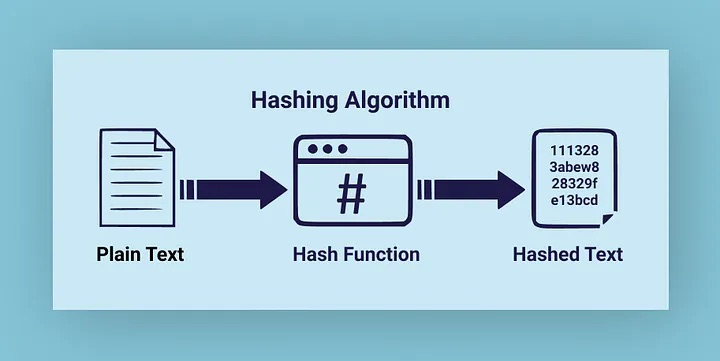
\includegraphics[width=0.5\textwidth]{img/1-img/hash-function.jpeg}
	\end{center}


\end{frame}

\begin{frame}
	\frametitle{Fefinizione funzione di hash}

	Dato un alfabeto $\mathfrak{A}$, indicheremo con $\mathfrak{A}^*$ l’insieme di tutte le stringhe finite di elementi di $\mathfrak{A}$

	\[
		\mathfrak{A}^* = \bigcup_{n \geq 1} \mathfrak{A}^n
	\]

	Tipicamente $\mathfrak{A} = \{0, 1\}$, e quindi $\mathfrak{A}^*$ è l’insieme di tutte le stringhe composte da bit.

	\vspace{1cm}
	Una funzione hash è una funzione $h : \mathfrak{A}^* \rightarrow \mathfrak{A}^n$ che mappa stringhe di lunghezza arbitraria in stringhe di lunghezza fissa $n$ (per esempio n = 160)

\end{frame}


\begin{frame}
	\frametitle{Proprietà delle funzioni di hash}

	\begin{itemize}
		\item \textbf{Determinismo}: per uno stesso input la funzione restituisce sempre lo stesso output.
		\item \textbf{Velocità}: la funzione deve essere veloce da calcolare.
		\item \textbf{Difficoltà di inversione}: data l'uscita della funzione è computazionalmente difficile trovare l'input.
		\item \textbf{Effetto valanga}: piccole variazioni nell'input devono produrre grandi variazioni nell'output.
		\item \textbf{Effetto valanga}: piccole variazioni nell'input devono produrre grandi variazioni nell'output.
		\item \textbf{Resistenza alle collisioni}: è computazionalmente difficile trovare due input diversi che producano lo stesso output.
	\end{itemize}
\end{frame}

\begin{frame}
	\frametitle{Preimage resistence}
	\textbf{Prima (debole) resistenza alla preimmagine}:
	\begin{itemize}
		\item per quasi tutti gli output pre-specificati, è computazionalmente infattibile trovare un qualsiasi input che venga hashato a quell'output.
		      Avendo \( y \), è difficile trovare un \( x \) tale che \( h(x) = y \).
	\end{itemize}
	\textbf{Seconda (forte) resistenza alla preimmagine}:
	\begin{itemize}
		\item per un input specificato, è computazionalmente infattibile trovare un altro input che produca lo stesso output.
		      Avendo \( x \), è difficile trovare un secondo input \( x' \neq x \) tale che \( h(x) = h(x') \).
	\end{itemize}

\end{frame}

\begin{frame}
	\frametitle{Secure Hash Algorithm: SHA-1}

	La specifica originale è stata pubblicata nel 1993 come \textbf{Secure Hash Standard} dal National Institute of Standards and Technology.
	SHA-0 fu ritirato dall'NSA e sostituito da una versione rivista dopo 2 anni quando fu pubblicato SHA-1 che prevedeva una rotazione di bit in più
	per correggere un difetto nell'algoritmo originale.

	\vspace{1cm}

	I digest prodotti da SHA-1 sono di \textbf{160 bit} e al massimo può elaborare messaggi di \textbf{2\textsuperscript{64} - 1} bit.
\end{frame}


\begin{frame}
	\frametitle{Secure Hash Algorithm: costruzione Merkle-Damgård}
	Le funzioni di hash come SHA-1, MD5 e SHA-2 sono basate sul costrutto di \textbf{Merkle-Damgård}, essi dimostrarono in modo indipndente
	che utilizando \textbf{un appropriato schema di padding} e la funzione di compressione è \textbf{resistente alle collisioni}, allora anche la \textbf{funzione di hash è resistente alle collisione}.

	\begin{center}
		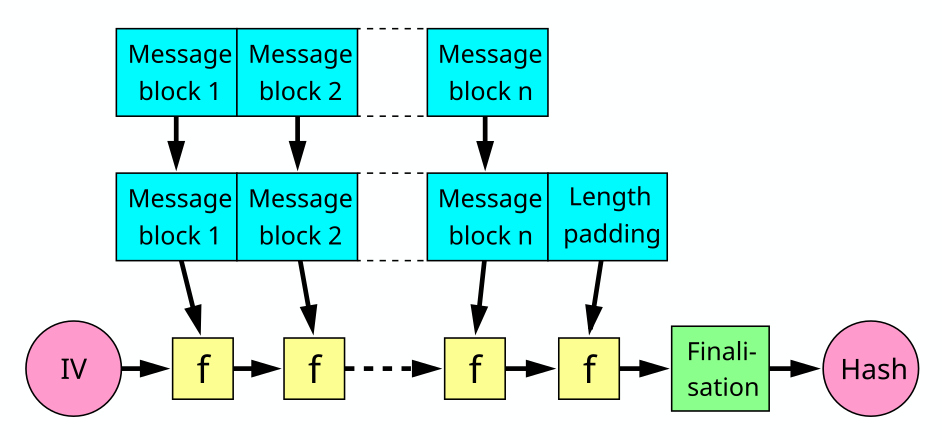
\includegraphics[width=0.8\textwidth]{img/1-img/Merkle-Damgard.png}
	\end{center}
\end{frame}


\begin{frame}
	\frametitle{Secure Hash Algorithm: Merkle-Damgård}

	Nel caso di SHA-1 l'input viene diviso in \textbf{blocchi da 512} bit che vengono processati uno alla volta.

	\vspace{1cm}


	Per fare in modo che la costruzione risultasse sicura, Merkle e Damgård proposero di
	riempire i messaggi con un padding che codificasse la lunghezza del messaggio originario (\textbf{rafforzamento di Merkle-Damgård}).
\end{frame}

\begin{frame}
	\frametitle{Secure Hash Algorithm: Elaborazione dei blocchi}

	\begin{columns}
		% Colonna a sinistra (Elenco)
		\begin{column}{0.6\textwidth}
			\begin{itemize}
				\item \textbf{Elaborazione dei blocchi tramite la funzione F}:
				      \begin{itemize}
					      \item F si occupa di trasformare 2 input di lunghezza fissa (blocco e stato) in un output di lunghezza fissa.
					      \item L'algoritmo parte con un vettore di inizializzazione VI di 160 bit.
					      \item In SHA-1 prima di elaborare il blocco esso viene suddiviso ed espanso in 80 parole da 32 bit.
				      \end{itemize}
			\end{itemize}
		\end{column}

		% Colonna a destra (Immagine)
		\begin{column}{0.4\textwidth}
			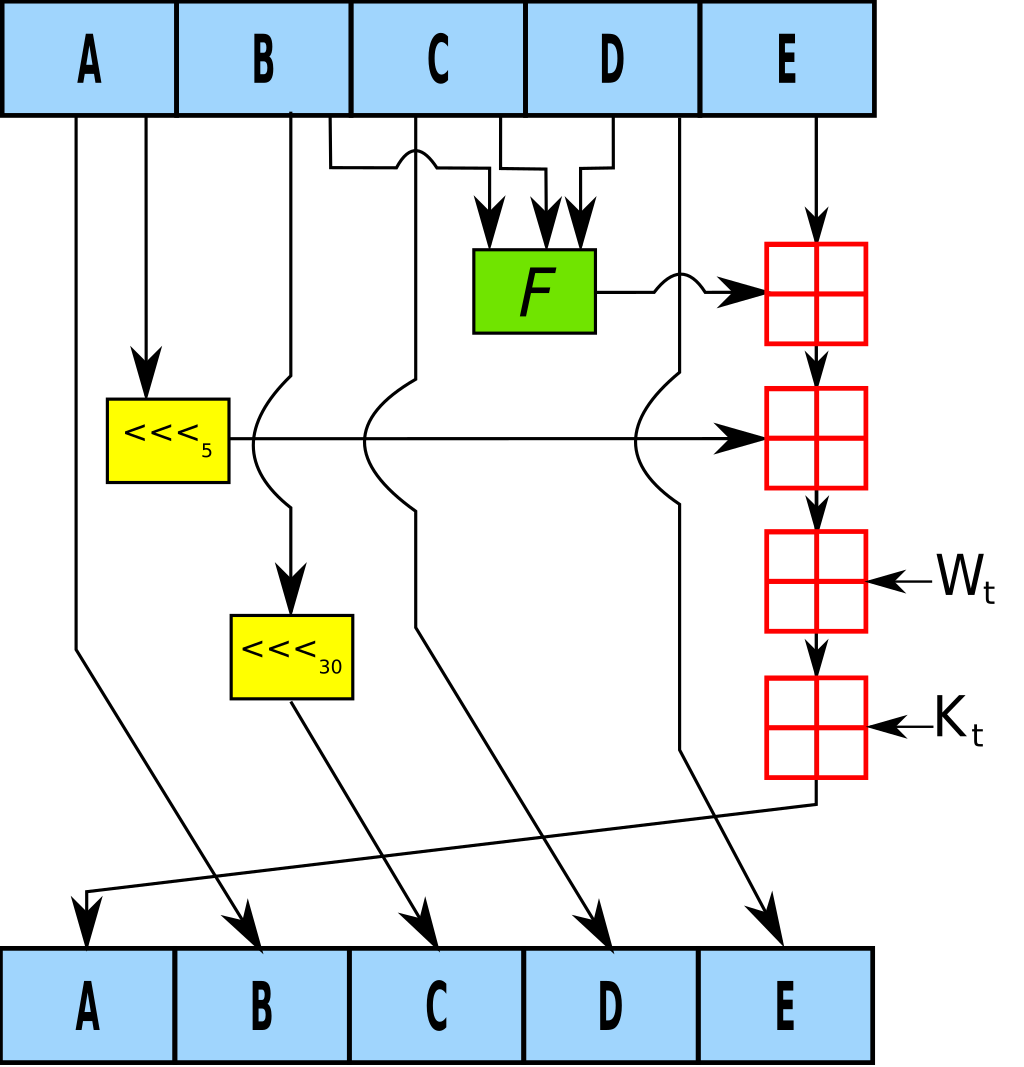
\includegraphics[width=\textwidth]{img/1-img/SHA-1.png}
		\end{column}
	\end{columns}

\end{frame}